
\section{Teorema de estabilidad}
En esta sección introduciremos el \emph{teorema de estabilidad de los diagramas de persistencia}, y profundizaremos en su demostración siguiendo \cite{Cohen-Steiner2007}. Primero estudiaremos la estabilidad para la \emph{distancia de Hausdorff}, y después, reforzaremos el resultado estudiando la estabilidad con la \emph{distancia bottleneck}.
\subsection{Proposición del teorema}
El teomera de estabilidad nos va a garantizar la robustez de los diagramas de persistencia. Dicho de otro modo, que ``pequeñas'' perturbaciones en las funciones, dan lugar a diagramas de persistencia ``cercanos''. Así pues, primero precisaremos el concepto de cercanía entre funciones y diagramas de persistencia.

Sean $X$ e $Y$ dos diagramas de persistencia. Recordamos que $X$ e $Y$ son dos multiconjuntos de puntos del plano extendido $\overline{\mathbb{R}}^2$, constituidos por un número finito de puntos sobre la diagonal, y por los puntos de la diagonal con multiplicidad infinito. 

\begin{definition}
Sean los puntos $p=(p_1, p_2)$ y $q=(q_1,q_2)$ en $\overline{\mathbb{R}}^2$. Entonces, la distancia infinito entre los puntos es:
\[
d_\infty(p, q)=\norm{p-q}_\infty= \max\{\abs{p_1 - q_1}, \abs{p_2-q_2}\}\,.
\]
\end{definition}

\begin{definition}
Sean $f,g: \mathbb{X} \to \mathbb{R}$ dos funciones continuas. Entonces, la distancia infinito entre las funciones es:
\[
d_\infty(f, g)=\norm{f-g}_\infty= \sup_{x\in \mathbb{X}}\ \abs{f(z) - g(x)}\,.
\]
\end{definition}

Definiremos las distancias Hausdorff y bottleneck sobre multiconjuntos (diagramas de persistencia en nuestro caso) de la siguiente forma
\begin{definition}
La \emph{distancia Hausdorff} y la \emph{distancia bottleneck} entre $X$ e $Y$ son, respectivamente
\begin{gather*}
H(X, Y) = \max\left\{ \adjustlimits\sup_{x\in X} \inf_{y\in Y} \norm{x-y}_\infty, \adjustlimits\sup_{y\in Y} \inf_{x\in X} \norm{y-x}_\infty \right\},\ \\
W_\infty(X, Y) = \adjustlimits\inf_{\eta: X \to Y} \sup_{x\in X} \norm{x-\eta(x)}_\infty
\end{gather*}
siendo $\eta: X \to Y$ las biyecciones de $X$ a $Y$.
\end{definition}
Las biyecciones entre dos diagramas de persistencia generan tres tipos de emparejamientos:
\begin{itemize}
	\item Ambos puntos fuera de la diagonal.
	\item Un punto fuera de la diagonal y otro en la diagonal.
	\item Ambos puntos en la diagonal.
\end{itemize}
Se puede observar que los puntos que determinar en mayor escala la distancia bottelneck son los del primer tipo, y los que menor importancia tienen son los del último tipo, ya que completarán el emparejamiento sin afectar en la distancia.

\begin{remark}
Debido a que la distancia bottleneck satisface una restricción adicional respecto a la distancia Hausdorff, es decir, la biyección entre los puntos; entonces, se cumple $H(X, Y) \leq W_\infty(X, Y)$.
\end{remark}

\begin{theorem}[Teorema de estabilidad para funciones tame]
Sea $\mathbb{X}$ un espacio topológico triangulable y sea $f,g: \mathbb{X} \to \mathbb{R}$ dos funciones tame continuas. Entonces, para cada dimensión $k$, la distancia bottleneck entre los diagramas de persistencia esta acotada por la distancia $L_\infty$ entre las funciones, es decir,
\[
W_\infty(\text{\rm Dgm}(f), \text{\rm Dgm}(g)) \leq \norm{f-g}_\infty\,.
\]
\end{theorem}

Luego, se garantiza que los diagramas de persistencia son estables bajo perturbaciones de baja amplitud. Este resultado se puede observar gráficamente en la figura \ref{ref:ejEstabilidad}, donde se observa que los valores críticos ``supérfluos'' de la función perturbada definen puntos en el diagrama muy próximos a la diagonal, y los valores críticos ``relevantes'' definen puntos muy próximos a los puntos del diagrama asociados a la función original.

\begin{figure}[!ht]
\centering
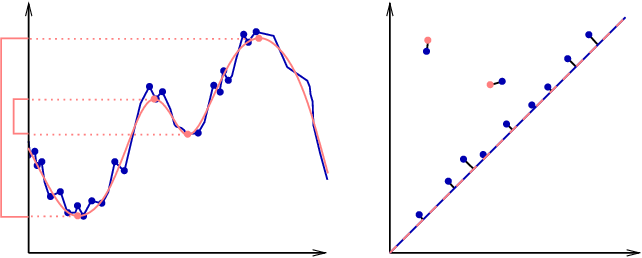
\includegraphics[width=0.8\textwidth]{include/figuras/estabilidadEj.png} 
\caption{A la izquierda se muestran dos funciones cercanas, una con muchos valores críticos y otra con cuatro. A la derecha se muestran los diagramas de persistencia superpuestos, con la biyección que da lugar a la distancia bottleneck. Fuente: \cite{Cohen-Steiner2007}}
\label{ref:ejEstabilidad}
\end{figure}  

\subsection{Estabilidad para la distancia Hausdorff}
\begin{theorem}[Teorema de estabilidad con la distancia Hausdorff para funciones tame]
Sea $\mathbb{X}$ un espacio topológico triangulable y sea $f,g: \mathbb{X} \to \mathbb{R}$ dos funciones tame continuas. Entonces, para cada dimensión $k$, la distancia Hausdorff entre los diagramas de persistencia esta acotada por la distancia $L_\infty$ entre las funciones, es decir,
\[
H(\text{\rm Dgm}(f), \text{\rm Dgm}(g)) \leq \norm{f-g}_\infty\,.
\]
\end{theorem}
\subsection{Estabilidad para la distancia bottleneck}
\todo{Subsección por hacer}
